
%(BEGIN_QUESTION)
% Copyright 2008, Tony R. Kuphaldt, released under the Creative Commons Attribution License (v 1.0)
% This means you may do almost anything with this work of mine, so long as you give me proper credit

The process trend shown below reveals a controller's response to the process variable signal and the setpoint.  The controller implements a full PID algorithm of the ``parallel'' type (equation shown below):

$$\includegraphics[width=15.5cm]{i04315x01.eps}$$

$$m = K_p e + {1 \over \tau_i} \int e \> dt + \tau_d {de \over dt}$$

Assuming each horizontal division is equal to 1 minute of time, determine the following tuning parameter values.  Be sure to show all your mathematical work!


\begin{itemize}
\item{} {\it Direct} or {\it Reverse} control action
\vskip 10pt
\item{} $K_p$ = \underbar{\hskip 50pt} (unitless gain)
\vskip 10pt
\item{} $\tau_i$ = \underbar{\hskip 50pt} minutes
\vskip 10pt
\item{} $\tau_d$ = \underbar{\hskip 50pt} minutes
\end{itemize}

\vskip 10pt

Finally, explain how we can tell this controller is {\it not} implementing either the ``Ideal'' (ISA) or ``Interactive'' (Series) PID equation, based solely on the trend graph.

\vfil 

\underbar{file i04315}
\eject
%(END_QUESTION)





%(BEGIN_ANSWER)

This is a graded question -- no answers or hints given!

%(END_ANSWER)





%(BEGIN_NOTES)

There is a conspicuous lack of both proportional and derivative actions evident in the trend.  This tells us $K_p$ and $\tau_d$ must both be set to zero.

The only active control action we see here is integral.  By definition, the number of minutes per repeat for an integral-only controller is the amount of time necessary for the output to ramp as far as the error, given a constant error over the integration interval.  Here, we may look at any ``flat'' portion where there is error between the PV and SP, then extrapolate from the output's ramp how long we would have to wait before the output ramps as far as the error.  During the periods of time where a 10\% error is maintained, the output ramps at a rate of 7.5\% every 4 minutes.  This equates to 5.333 minutes to ramp 10\% (the same magnitude as the error).

\vskip 10pt

\begin{itemize}
\item{} {\bf Direct} control action
\vskip 10pt
\item{} $K_p$ = {\bf 0} (unitless gain)
\vskip 10pt
\item{} $\tau_i$ = {\bf 5.333} minutes
\vskip 10pt
\item{} $\tau_d$ = {\bf 0} minutes
\end{itemize}

\vskip 10pt

We can tell the controller equation must be ``Parallel'' because there is zero proportional action.  If it were implementing either the ISA or the Series equation, a proportional gain of zero will kill the I and D responses as well!

%INDEX% Control: determining P, I, D from graph of controller response

%(END_NOTES)


